%-------------------------------------------
% En-tête type de document pour le projet PLD
% Il suffit de remplir le input ligne 45
%-------------------------------------------

\documentclass[a4paper]{article}

\usepackage[utf8]{inputenc}
\usepackage[top=2cm, bottom=2cm, left=2cm, right=2cm]{geometry}
\usepackage{ucs}
% Reconnaitre les caratères accentués dans le source.
\usepackage[T1]{fontenc}
\usepackage{lmodern}
\usepackage[francais]{babel}
% Insertion d'images
\usepackage{graphicx}
% Utilisation du symbole EURO
\usepackage{eurosym}

\setlength{\parskip}{10pt plus 1pt minus 1pt}

\begin{document}

%------------------------------------- Page de titre
\begin{titlepage}
~
\vfill
\begin{center}
\begin{Huge}
Projet Fouille de Données\\ Les communes de la région Rhône-Alpes \end{Huge}
\vfill
\\Quentin \bsc{Calvez}, Xavier \bsc{Sauvagnat}\\
\vfill
\begin{Large}
Mars 2012
\end{Large}
\vfill
\begin{tabular}{|c|c|c|c|c|}
  \hline
   Destinataire & Version & Etat & Dernière révision \\
   \hline
   Mr. Bouliquot & 1 & Validé & \today \\
   \hline
\end{tabular}
\end{center}
\vfill
\end{titlepage}
%----------------------------------------------------
%--------------------------------- Table des matières
\newpage
\tableofcontents
\newpage
%----------------------------------------------------

%------------------- Insertion du contenu du document
\section{Introduction}

Nous allons dans ce document présenter notre analyse et traitement d'un jeu de données qui nous a été fournis, contenant des informations sur les 293 communes du département du Rône. Nous verrons tout d'abord en détails quelles sont les données que l'on nous a fournis, quelles autres informations nous avons pu leur adjoindre afin de faciliter leur analyse. On se concentrera ensuite sur la technique utilisée et les résultats que nous avons obtenus, étape par étape.

\section{Jeux de données}

\subsection{Jeu original}

Le jeu de données qui nous était fournis nous a servi de base dans notre recherche. Il propose des données démographiques telles que les taux de naissances/décès, des informations sur les revenus, sur le nombre de foyers, et sur la présence ou non de certaines industries. Le tout par commune.

\subsection{Coordonnées GPS IGN}

Afin de mieux visualiser le jeu original dans l'espace, nous lui avons adjoint les coordonnées GPS de chaque commune, nous permettant ainsi de placer sur une carte les communes et de pouvoir comparer leur emplacement avec d'autres de leurs caractéristiques.

\subsection{Recensement INSEE}
Bien qu'il soit indiqué dans les variables qu'il y est une estimation de la population en 2006, ces données sont absentes du jeu de base, nous avons donc rajouté des informations démographiques provenant d'un recensement de 2008 effectué par l'INSEE et qui nous permettent de connaître le nombre d'habitant total par commune, tout en ajoutant une nouvelle dimension qui est la classification de ces effectifs par tranches d'âge.

\section{Analyse}

\subsection{Considération sur les domaines d'activité}

 Nous allons commencer par une exploration basique des données afin de tirer des conclusions ou plutôt vérifier que nous manipulons les données correctement.

La chaîne de composant ci-dessous permet de créer un affichage de "boîtes à moustaches" pour les différents domaines d'activités, à savoir le service, le commerce, la construction et l'industrie.
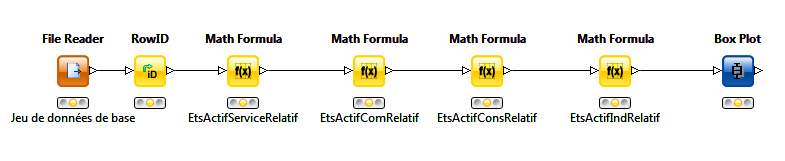
\includegraphics{png/BoxPlotDomainesActivité_knime.png}

Pour calculer le pourcentage que réprésente un secteur d'activité, nous avons utlisé le composant \textit{Math Formula}, qui nous permet de faire des calculs mathématiques avec les valeurs des attributs. Dans notre cas, pour le calcul du pourcentage d'établissement de service dans une commune, il suffit de diviser le nombre d'établissements actifs de service par le nombre total d'établissements actifs.
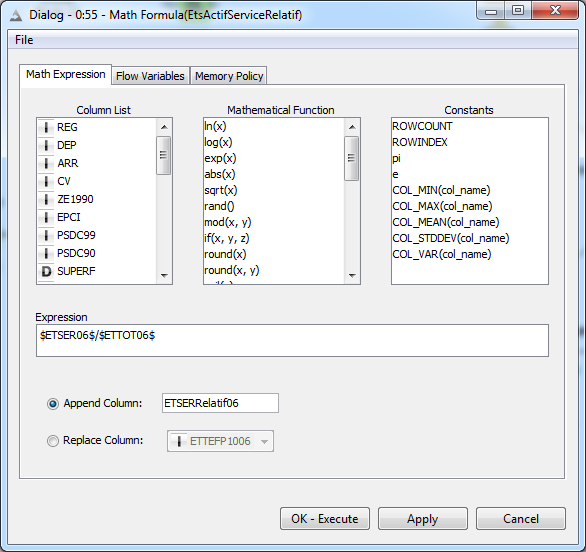
\includegraphics{png/MathFormulaEtsActifServiceRelatif.png}

On obtient le graphique suivant, avec les "boites à moustaches" pour les différents domaines d'activité. Cela permet de mettre en évidence que les communes du département du Rhône ont majoritairement des établissements de service, ce qui n'est pas étonnant. On remarquera que nous avons quelques valeurs exceptionnelles, notamment la commune de Riverie, qui compte 94% d'établissement de service, mais il s'agit d'une des plus petits communes du département en taille et nombre d'habitants, il faut donc relativiser l'importance de l'activité de service.
D'ailleurs un certains nombre de communes ne comptent pas d'établissement de construction ou d'industrie, ce qui n'est guère étonnant vue la petite taille de certaines d'entre elles. Pour les établissements de commerces, la valeur 0% est mise en dehors du premier quartile, mais on ne peut malgré tout pas considérer cela comme une valeur extraordinaire.
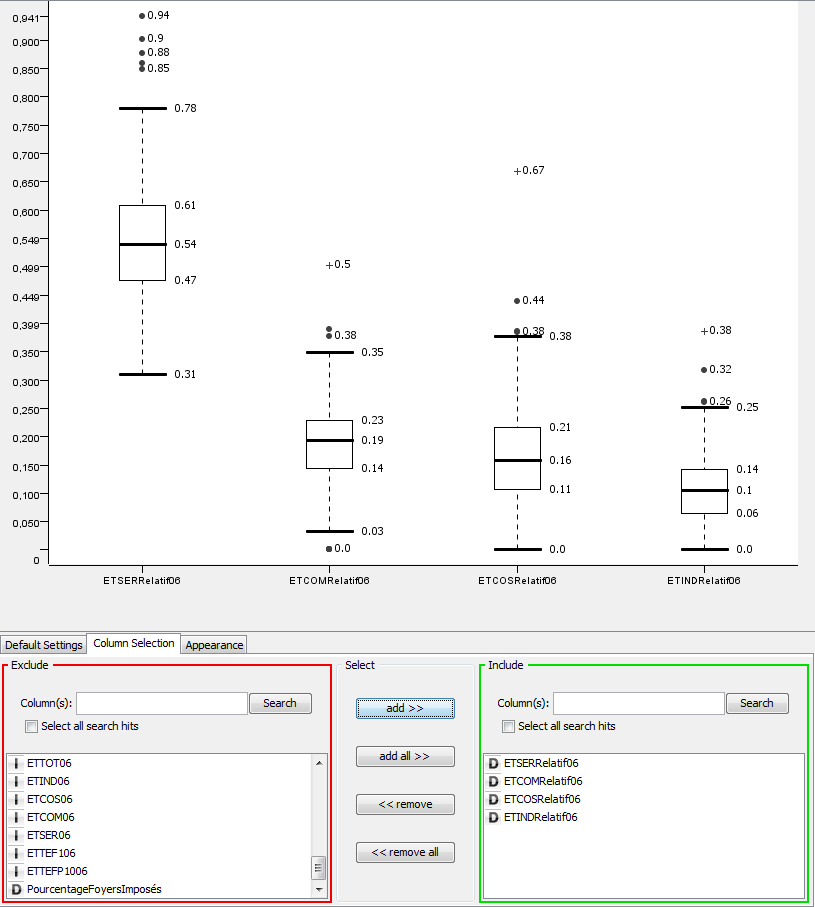
\includegraphics{png/BoxPlotDomainesActivité.png}

{subsection{Considération sur la densité de population}
Nous allons utiliser un outil plus puissant offert par Knime afin d'analyser les données: la clusterisation grâce à  l'algorithme k-Means. Nous n'appliquerons la clusterisation que sur un seul paramètre dans ce cas.

Nous avons adjoint les coordonnées géographiques de chaque commune afin de pouvoir obtenir une réprésentation spatiale réaliste. La clusterisation n'étant pas fait sur des critéres géographiques, cela nous permet de voir si les groupements qui apparaissent se retrouve sur une carte, car la position d'une commune fait pleinement partie de son identité.
Nous avons également ajouté un jeu de données sur la population totale (sans double compte) de chaque commune datant de 2008,car la variable POPEST06 ( Population totale estimée en 2006) est absente du jeu de données de base, celle des données datant de 1999 sont disponibles. 

Le workflow utilisé est le suivant:
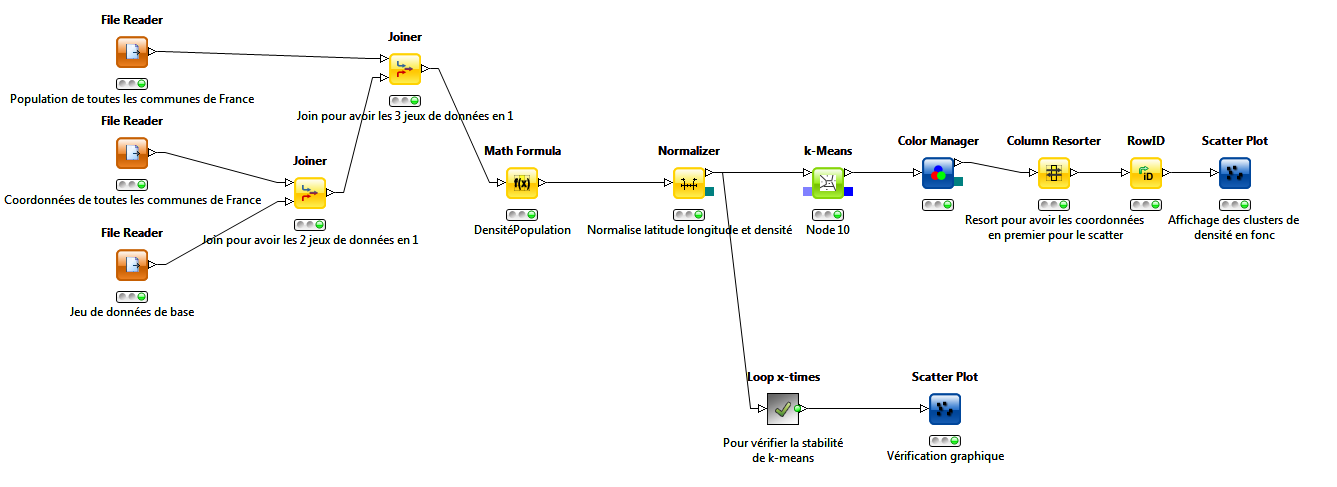
\includegraphics{png/Clusterisation en fonction de la densité de population.png}

Le cluster obtenu est le suivant:
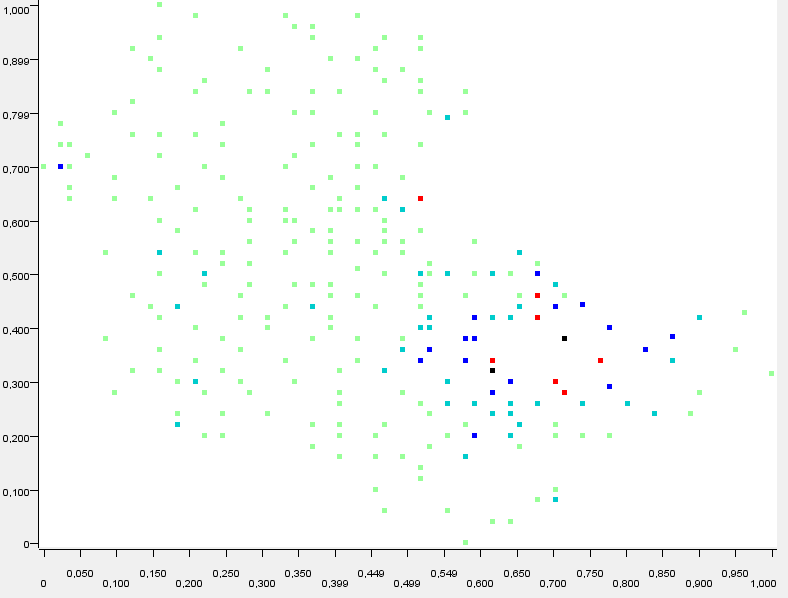
\includegraphics{png/Clusters en fonction de la densité de population.png}

On remarque que la densité est plus importante dans le périphérie de Lyon et Villeurbanne, avec une décroissance plus on s'éloigne. Villefranche-sur-Saône, situé sur la frontière entre l'Ain et le Rhône, se démarque part sa forte densité dûe à sa forte activité.

Nous avons également vérifier la stabilité de notre clusterisation en comparant simplement la taille des clusters entre les différentes intérations. C'est le moyen le plus simple pour faire une vérification, pour plus de précision, il faudrait également vérifier que ce sont bien les mêmes éléments qui composent les clusters.
\includegraphics{png/Outil de vérification de la clusterisation en fonction de la densité de population.png}

Suivant les différentes intérations, nous obtenons bien des clusters de même taille, nous supposerons donc qu'il s'agit des mêmes.
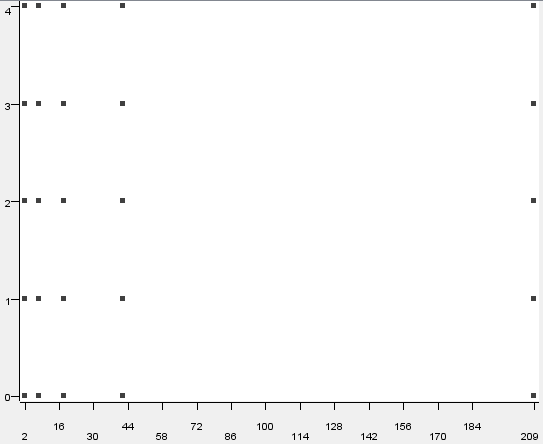
\includegraphics{visualisation de la stabilité de la clusterisation en fonction de la densité de population.png}

\section{Conclusion}
%----------------------------------------------------

%-------------------

%----------------------------------------------------
\end{document}